\chapter{Evaluation and Analysis of GPU Communication}\label{eval}
This chapter examines analysis results of the traces generated with the technique described in chapter \ref{chap:impl}. The analysis is sectioned into several tiers, as described in \ref{methodik:methods}.\\


\section{Evaluated Applications}
The evaluated application are listed in table \ref{eval-apps}. The applications are selected to represent typical problem Domains in scientific computing. 
\begin{table}[h]
	\centering
\begin{tabular}{|l|c|c|c|}
	\hline 
	Application & Source & Domain & Abbreviation \\ 
	\hline 
	Histogram64 & CUDA SDK & Histogram & hist \\ 
	\hline 
	Hotspot 2D & Rodinia Benchmark & 2D Stencil & hs2d \\ 
	\hline 
	Hotspot 3D & Rodinia Benchmark & 3D Stenceil & hs3d \\ 
	\hline 
	Pathfinder & Rodinia Benchmark & Pathfinder & path \\ 
	\hline 
	Breadth First Seach & Rodinia Benchmark & Graphs & bfs \\ 
	\hline 
	NBody & ZiTi CEG & Particle Dynamics & nbody \\ 
	\hline 
\end{tabular} 
\caption{Application used for communication evaluation}
\label{eval-apps}
\end{table}
\textit{Hist}, \textit{hs2d}, \textit{hs3d} and \textit{nbody} are more regular applications, where each CTA only operates within his data region. \textit{BFS} and \textit{path} tend to more irregularity, as the execution is more dynamic and the behaviour is more depended on the input data. 
\section{Tier I Analysis}
\subsection{Communication Fraction}
This metric displays the fraction of communication, compared to the total data written by an application. Figure \ref{com-ratio} directly compared all applications and shows that for all of them, at least 30\% of all writes is accessed by another CTA or another kernel in following iterations.

\textit{Nbody} and \textit{hist} show a very high ratio of communication, because \textit{nbody} is an $n$-to-$n$ problem and the histogram algorithm reduces a problem into bins, only using on the data generated in the preceding step. The more irregular applications, \textit{bfs} and \textit{path}, communicate less data compared to the four regular applications.
\begin{figure}[t]
	\centering
	\includegraphics[width=\textwidth]{../../../Global-Memory-Tracing/memtrace-pass/plots/write-com-ratio}
	\caption{Ration of communication to total of all writes.}
	\label{com-ratio}
\end{figure}
\subsection{Transfer Size CDF}
Figure \ref{fig:CDF} shows the cumulative distribution functions (CDF) plots for each application. The CDF shows the cumulative probability of a transfer size between two CTAs to occur during the execution. All applications, except \textit{path}, show one or few dominating transfer sizes. The \textit{path} application shows two slopes with linear rising probability for a range of transfer sizes.

\begin{figure}[t]
%	\begin{subfigure}[b]{0.45\textwidth}
%		\includegraphics[width=1\linewidth]{../../../Global-Memory-Tracing/memtrace-pass/plots/cdf/bfs}
%		\caption{BFS}
%		\label{fig:cfd-bfs}
%	\end{subfigure}
%	\begin{subfigure}[b]{0.45\textwidth}
%		\includegraphics[width=1\linewidth]{../../../Global-Memory-Tracing/memtrace-pass/plots/cdf/hist}
%		\caption{Histogram}
%		\label{fig:density-hist}
%	\end{subfigure}
%	\begin{subfigure}[b]{0.45\textwidth}
%		\includegraphics[width=1\linewidth]{../../../Global-Memory-Tracing/memtrace-pass/plots/cdf/hs2d}
%		\caption{Hotspot 2D}
%		\label{fig:cfd-hs2d}
%	\end{subfigure}
%	\begin{subfigure}[b]{0.45\textwidth}
%		\includegraphics[width=1\linewidth]{../../../Global-Memory-Tracing/memtrace-pass/plots/cdf/hs3d}
%		\caption{Hotspot 3D}
%		\label{fig:cfd-hs3d}
%	\end{subfigure}
%	\begin{subfigure}[b]{0.45\textwidth}
%		\includegraphics[width=1\linewidth]{../../../Global-Memory-Tracing/memtrace-pass/plots/cdf/path}
%		\caption{Pathfinder}
%		\label{fig:cfd-path}
%	\end{subfigure}
%	%add desired spacing between images, e. g. ~, \quad, \qquad, \hfill etc. 
%	%(or a blank line to force the subfigure onto a new line)
%	\hfill
%	\begin{subfigure}[b]{0.45\textwidth}
%		\includegraphics[width=1\linewidth]{../../../Global-Memory-Tracing/memtrace-pass/plots/cdf/nbody}
%		\caption{NBody}
%		\label{fig:cfd-nbody}
%	\end{subfigure}
	\includegraphics[width=\textwidth]{../../../Global-Memory-Tracing/memtrace-pass/plots/combined-cfd}
	\caption{Message Size CDF Plots}
	\label{fig:CDF}
\end{figure}
\subsection{Density Map}
The density plots, sometimes called heatmap, describes the frequency of CTA interaction across BSP supersteps. The x-Axis are the CTAs performing writes, the y-Axis are the follow-up reads to each write. Different kernels in an application are ignored, and only the CTA ID is used to identify communciation partners. Figure \ref{fig:density-plots} displays a subset of 200 CTAs for each application. The IDs of all CTA are serialized in $x$,$y$,$z$ order, $x$ being the most dominant dimension. 

The regular applications show highly regular frequency patterns. The irregular applications show two very different patters. \textit{Path} has only few partners and the frequency varies significantly. \textit{Bfs} shows two extremes, high frequency with high regularity and low frequency with low regularity.
The first extreme is caused by two kernels alternating during the iterations, where CTAs with the same ID process the same segment of the graph.  Latter is caused by the frontier array, used at the segment borders. A different graph would create the same pattern of the first extreme, but a different pattern of the second extreme.

As the CDF plot shows, all applications are dominated by few transfer sizes between CTAs, the patterns in figure \ref{fig:density-plots} would remain largely unchanged if the density was replaced with accumulated data volumes.
\begin{figure}[h!]
	\begin{subfigure}[b]{0.45\textwidth}
		\includegraphics[width=1\linewidth]{../../../Global-Memory-Tracing/memtrace-pass/plots/heatmap/bfs}
		\caption{BFS}
		\label{fig:density-bfs}
	\end{subfigure}
	\begin{subfigure}[b]{0.45\textwidth}
		\includegraphics[width=1\linewidth]{../../../Global-Memory-Tracing/memtrace-pass/plots/heatmap/hist}
		\caption{Histogram}
		\label{fig:density-hist}
	\end{subfigure}
	\begin{subfigure}[b]{0.45\textwidth}
		\includegraphics[width=1\linewidth]{../../../Global-Memory-Tracing/memtrace-pass/plots/heatmap/hs2d}
		\caption{Hotspot 2D}
		\label{fig:density-hs2d}
	\end{subfigure}
	\begin{subfigure}[b]{0.45\textwidth}
		\includegraphics[width=1\linewidth]{../../../Global-Memory-Tracing/memtrace-pass/plots/heatmap/hs3d}
		\caption{Hotspot 3D}
		\label{fig:density-hs3d}
	\end{subfigure}
	\begin{subfigure}[b]{0.45\textwidth}
		\includegraphics[width=1\linewidth]{../../../Global-Memory-Tracing/memtrace-pass/plots/heatmap/path}
		\caption{Pathfinder}
		\label{fig:density-path}
	\end{subfigure}
	%add desired spacing between images, e. g. ~, \quad, \qquad, \hfill etc. 
	%(or a blank line to force the subfigure onto a new line)
	\hfill
	\begin{subfigure}[b]{0.45\textwidth}
		\includegraphics[width=1\linewidth]{../../../Global-Memory-Tracing/memtrace-pass/plots/heatmap/nbody}
		\caption{NBody}
		\label{fig:density-nbody}
	\end{subfigure}
	\caption{Transfer Density Plots}
	\label{fig:density-plots}
\end{figure}
%\subsection{Volume Map}
%\begin{figure}
%	\begin{subfigure}[b]{0.45\textwidth}
%		\includegraphics[width=1\linewidth]{../../../Global-Memory-Tracing/memtrace-pass/plots/heatmap-vol/bfs}
%		\caption{BFS}
%		\label{fig:volume-bfs}
%	\end{subfigure}
%	\begin{subfigure}[b]{0.45\textwidth}
%		\includegraphics[width=1\linewidth]{../../../Global-Memory-Tracing/memtrace-pass/plots/heatmap-vol/hist}
%		\caption{Histogram}
%		\label{fig:volume-hist}
%	\end{subfigure}
%	\begin{subfigure}[b]{0.45\textwidth}
%		\includegraphics[width=1\linewidth]{../../../Global-Memory-Tracing/memtrace-pass/plots/heatmap-vol/hs2d}
%		\caption{Hotspot 2D}
%		\label{fig:volume-hs2d}
%	\end{subfigure}
%	\begin{subfigure}[b]{0.45\textwidth}
%		\includegraphics[width=1\linewidth]{../../../Global-Memory-Tracing/memtrace-pass/plots/heatmap-vol/hs3d}
%		\caption{Hotspot 3D}
%		\label{fig:volume-hs3d}
%	\end{subfigure}
%	\begin{subfigure}[b]{0.45\textwidth}
%		\includegraphics[width=1\linewidth]{../../../Global-Memory-Tracing/memtrace-pass/plots/heatmap-vol/path}
%		\caption{Pathfinder}
%		\label{fig:volume-path}
%	\end{subfigure}
%	%add desired spacing between images, e. g. ~, \quad, \qquad, \hfill etc. 
%	%(or a blank line to force the subfigure onto a new line)
%	\hfill
%	\begin{subfigure}[b]{0.45\textwidth}
%		\includegraphics[width=1\linewidth]{../../../Global-Memory-Tracing/memtrace-pass/plots/heatmap/nbody}
%		\caption{NBody}
%		\label{fig:volume-nbody}
%	\end{subfigure}
%	\caption{Transfer Volume Plots}
%	\label{fig:animals}
%\end{figure}

\subsection{CTA In/Out-Degree}
The in and out degree describe the number  communication partners, separated between incoming and outgoing transfers, for each CTA. Figure \ref{fig:Cta-degree} plots the percentages of selected bins for each application. 

Except for \textit{nbody}, and to a smaller degree \textit{bfs} and \textit{path}, no application performs point-to-point communication. Almost every communication happening is, to some degree, a collective communication.

Most applications show low variance, and the in- and out-degree, and few communication partners. Notable are \textit{hist} and \textit{bfs}, which have higher number of communication partners and \textit{bfs} also shows a stronger variance of in- and out-degrees. Also notable is that although \textit{path} is a dynamic application, the number of communication partners is steady.

\begin{figure}[h!]
%	\begin{subfigure}[b]{0.45\textwidth}
%		\includegraphics[width=1\linewidth]{../../../Global-Memory-Tracing/memtrace-pass/plots/com-degree/bfs}
%		\caption{BFS}
%		\label{fig:deg-bfs}
%	\end{subfigure}
%	\begin{subfigure}[b]{0.45\textwidth}
%		\includegraphics[width=1\linewidth]{../../../Global-Memory-Tracing/memtrace-pass/plots/com-degree/hist}
%		\caption{Histogram}
%		\label{fig:deg-hist}
%	\end{subfigure}
%	\begin{subfigure}[b]{0.45\textwidth}
%		\includegraphics[width=1\linewidth]{../../../Global-Memory-Tracing/memtrace-pass/plots/com-degree/hs2d}
%		\caption{Hotspot 2D}
%		\label{fig:deg-hs2d}
%	\end{subfigure}
%	\begin{subfigure}[b]{0.45\textwidth}
%		\includegraphics[width=1\linewidth]{../../../Global-Memory-Tracing/memtrace-pass/plots/com-degree/hs3d}
%		\caption{Hotspot 3D}
%		\label{fig:deg-hs3d}
%	\end{subfigure}
%	\begin{subfigure}[b]{0.45\textwidth}
%		\includegraphics[width=1\linewidth]{../../../Global-Memory-Tracing/memtrace-pass/plots/com-degree/path}
%		\caption{Pathfinder}
%		\label{fig:deg-path}
%	\end{subfigure}
%	%add desired spacing between images, e. g. ~, \quad, \qquad, \hfill etc. 
%	%(or a blank line to force the subfigure onto a new line)
%	\hfill
%	\begin{subfigure}[b]{0.45\textwidth}
%		\includegraphics[width=1\linewidth]{../../../Global-Memory-Tracing/memtrace-pass/plots/com-degree/nbody}
%		\caption{NBody}
%		\label{fig:deg-nbody}
%	\end{subfigure}
	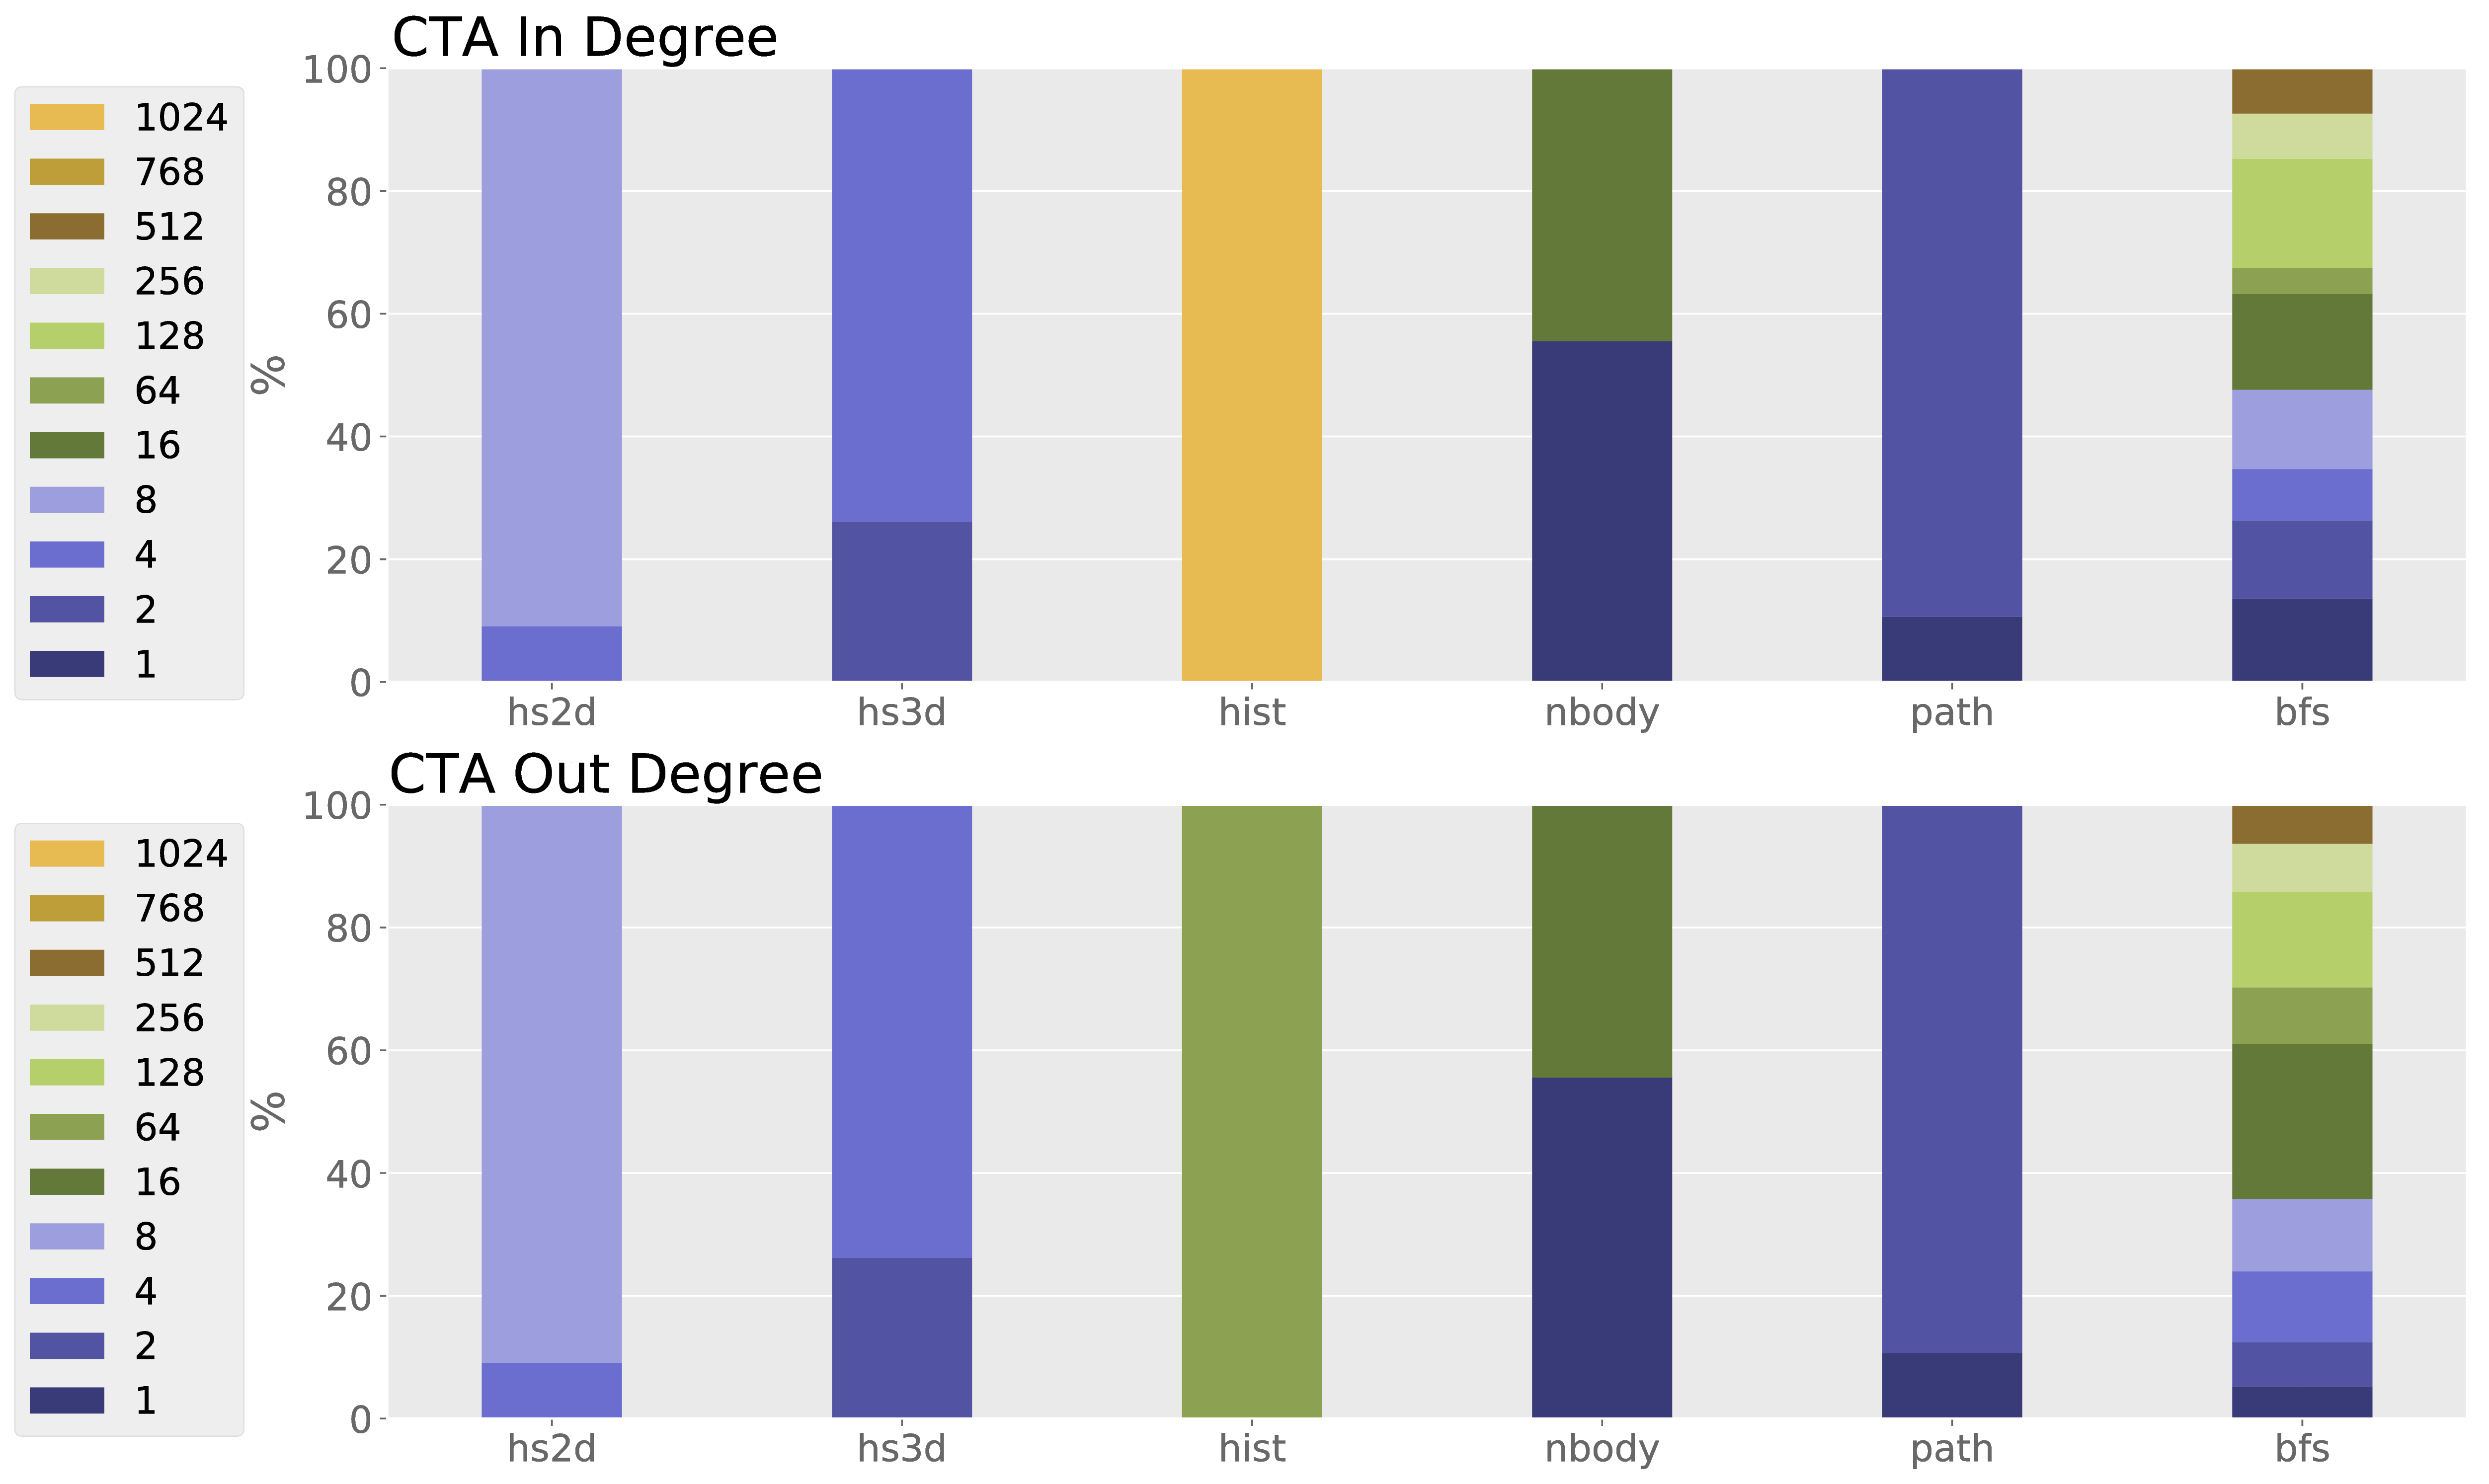
\includegraphics[width=\textwidth]{../../../Global-Memory-Tracing/memtrace-pass/plots/cta-degree}
	\caption{Number of incoming and outgoing communication partners of each CTA}
	\label{fig:Cta-degree}
\end{figure}
\subsection{Bisection Volume}
This metric shows the data volume moved a hypothetical cut in each dimension. The cut creates two equal halfs. Most applications only use the $x$ dimension, so the other dimensions are 0.
\begin{figure}[t]
	\centering
	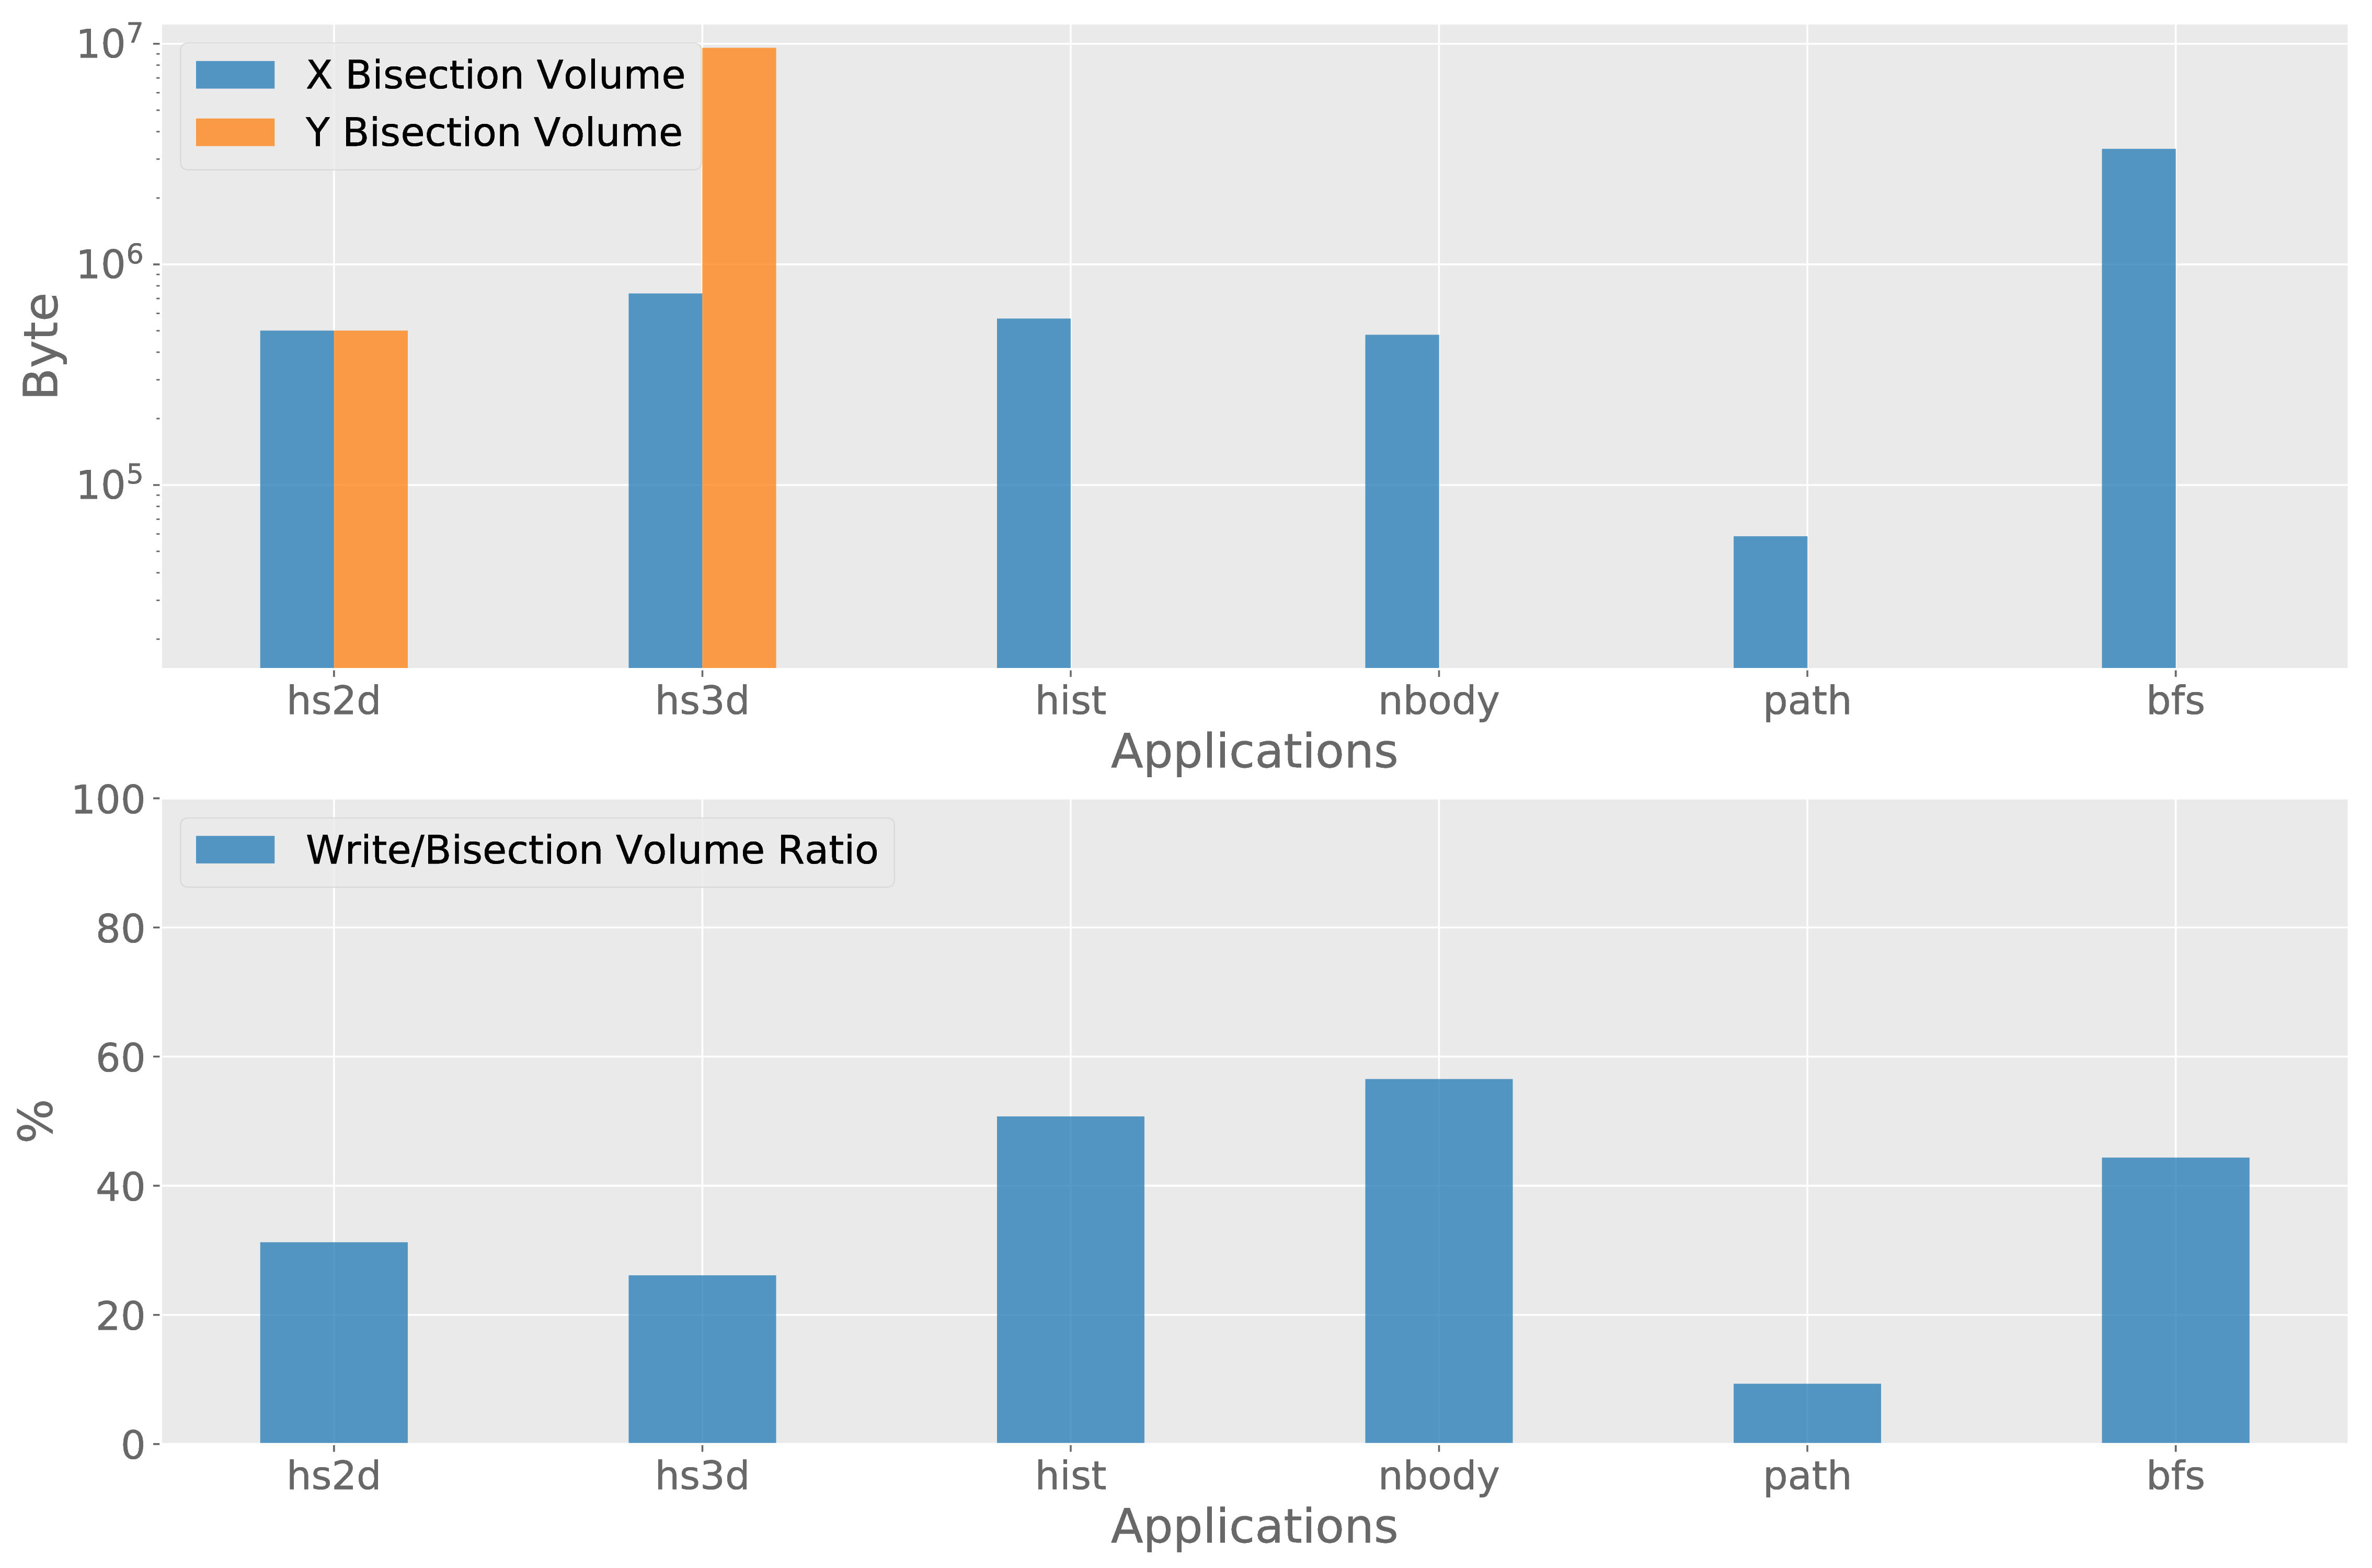
\includegraphics[width=\textwidth]{../../../Global-Memory-Tracing/memtrace-pass/plots/bisection-volume}
	\caption{Bisection Volume}
	\label{bisection-vols}
\end{figure}
\subsection{Communication Stride}
The stride in loads and stores involved in communication can be a critical aspect for performance. Large strides reduce the available memory bandwidth and increase latency.
\begin{figure}[t]
	\centering
	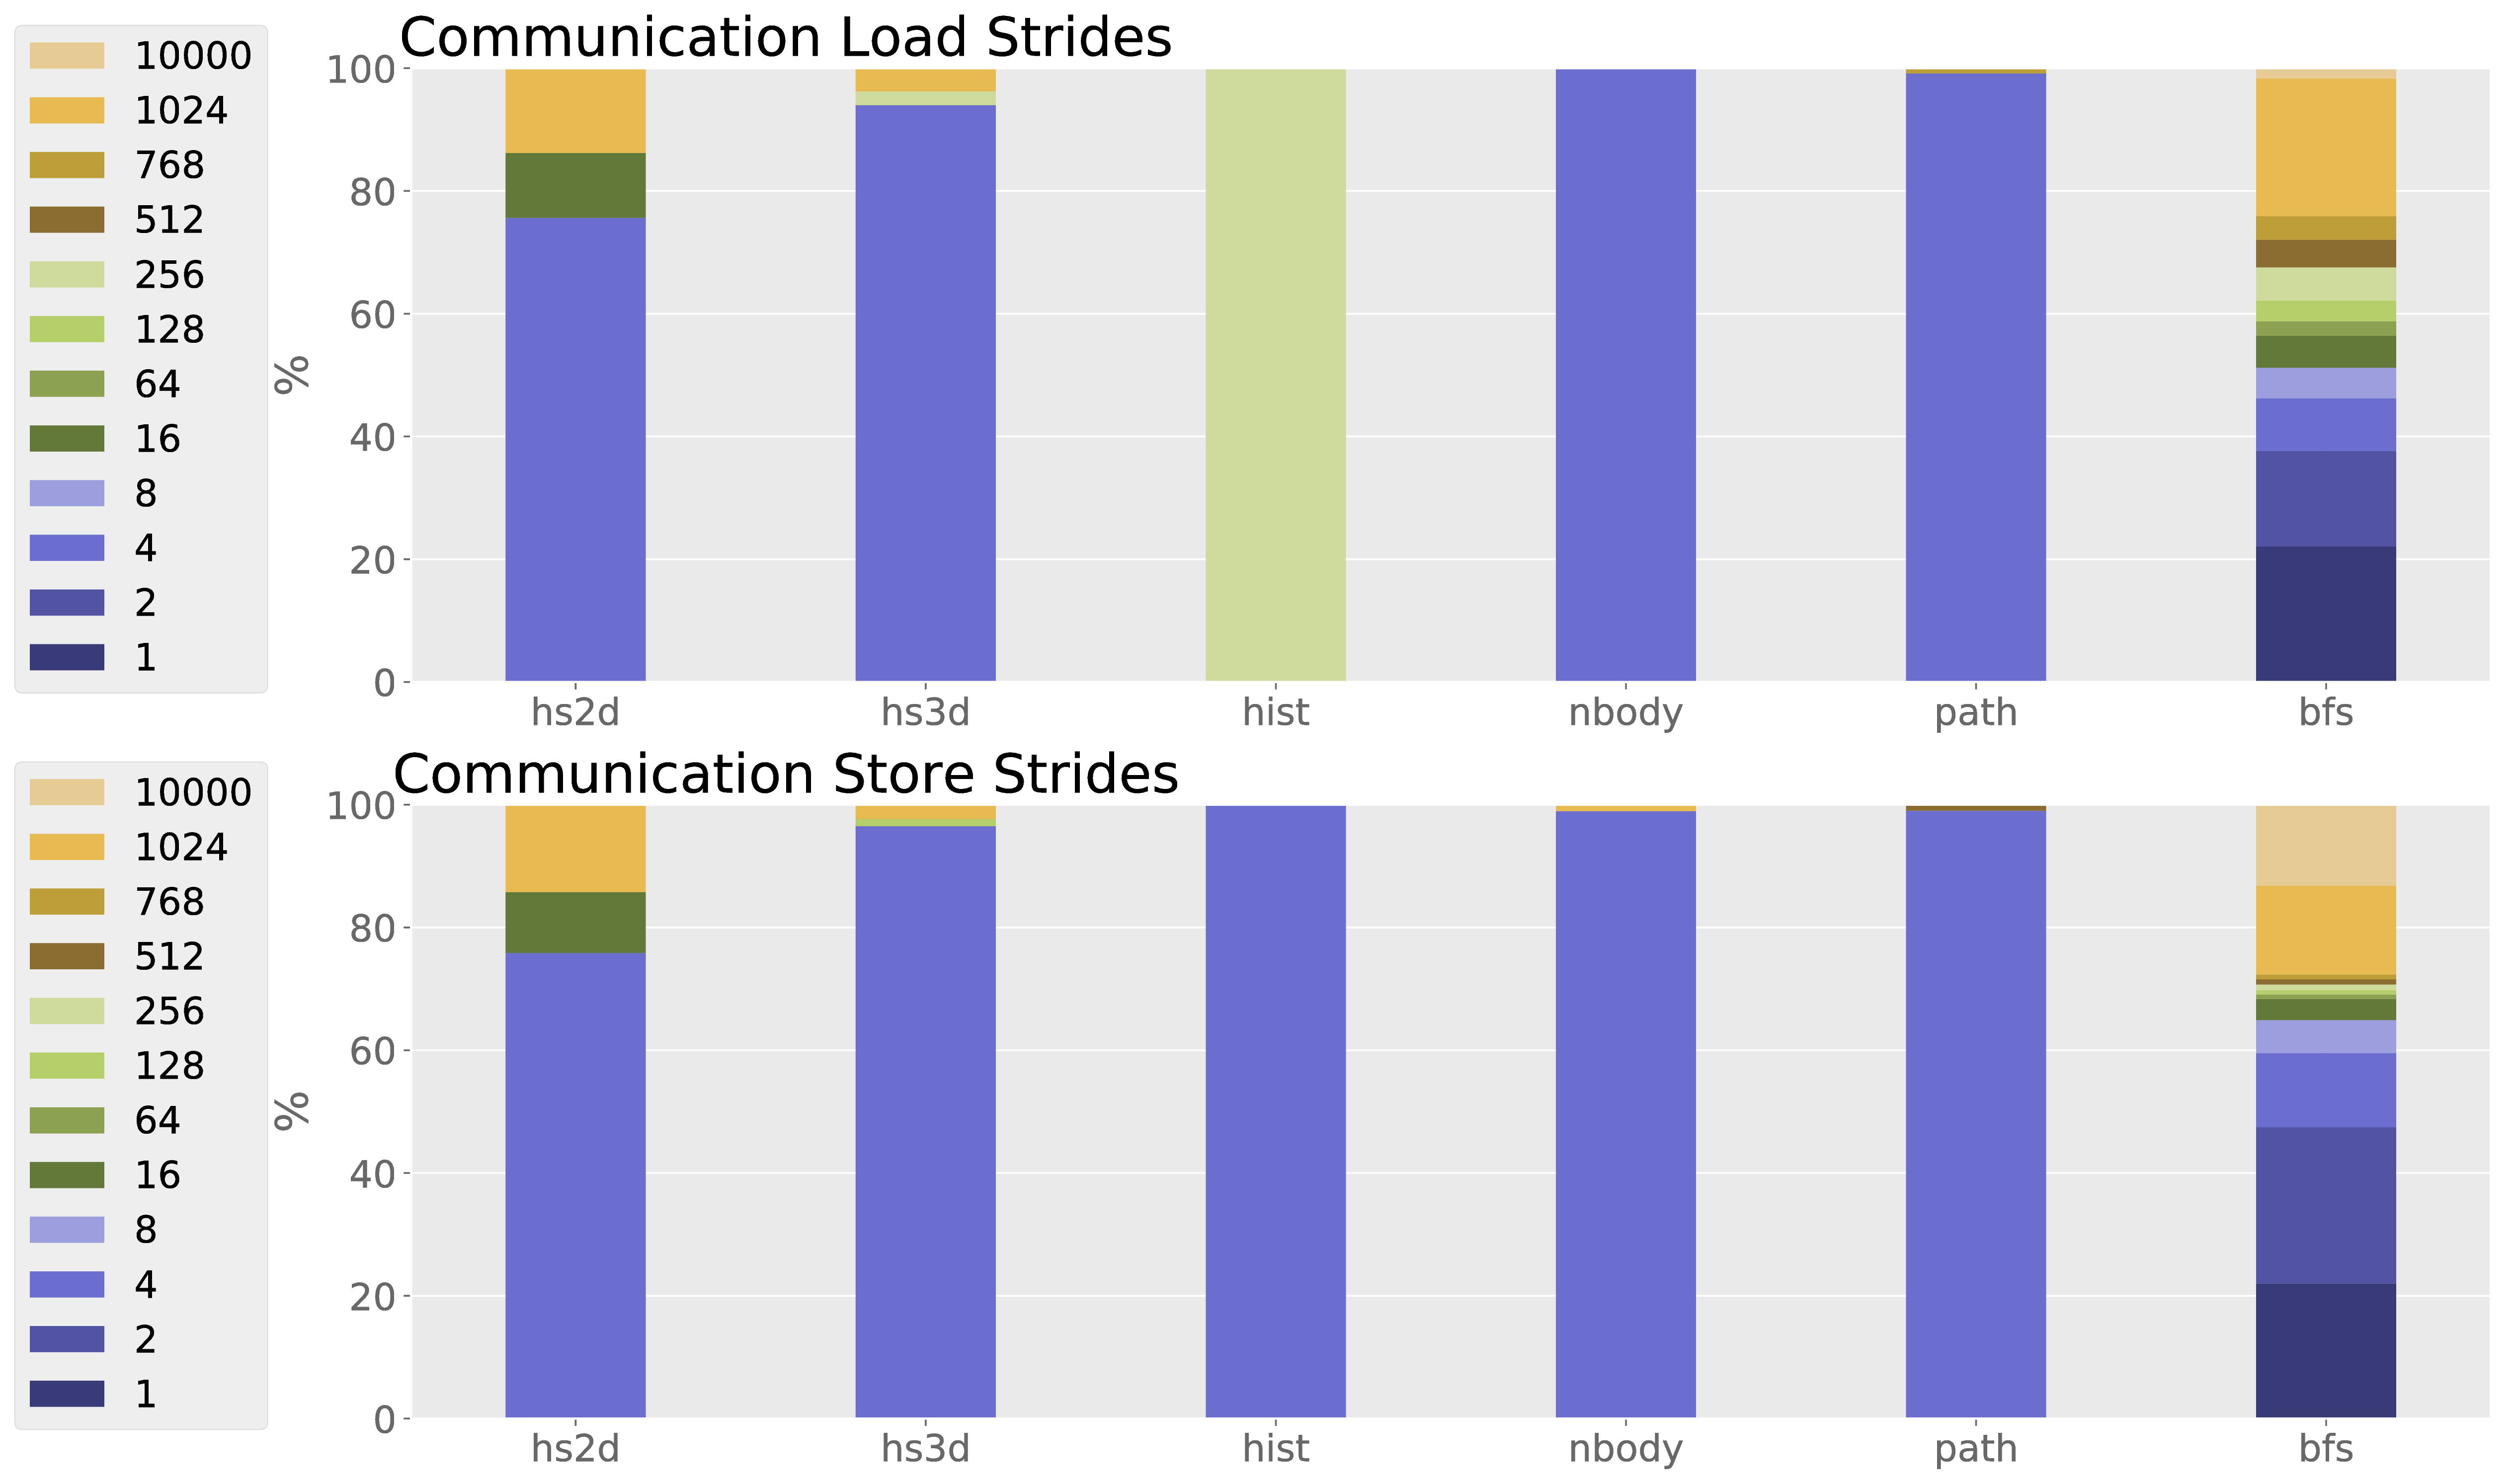
\includegraphics[width=\textwidth]{../../../Global-Memory-Tracing/memtrace-pass/plots/strides}
	\caption{Communication Stride}
	\label{com-stride}
\end{figure}
\newpage
\section{Tier II Analysis}
\subsection{Kernel communication Evolution}
This analysis shows how the data volumes change across supersteps. It is separated into loads and stores. Loads start at superstep one because as to our definition of communication, there can be no load that is part
of communication during the first superstep. Stored end before Loads, because the last store of an application is no communication, either.

The graph is to read as such: Stores happened in this superstep and are readable in the next. Loads read data from the preceding superstep. CTA in- and out degree analysis showed, every communication is happening in a collective environment. This means that there is no simple single writer, single reader matching across supersteps, which is the reason loads and stores are separated in this graphs.

The zig-zag like patterns for some applications are the result of different kernels alternating during
execution.

The data volumes remain 
\begin{figure}[t]
	\centering
	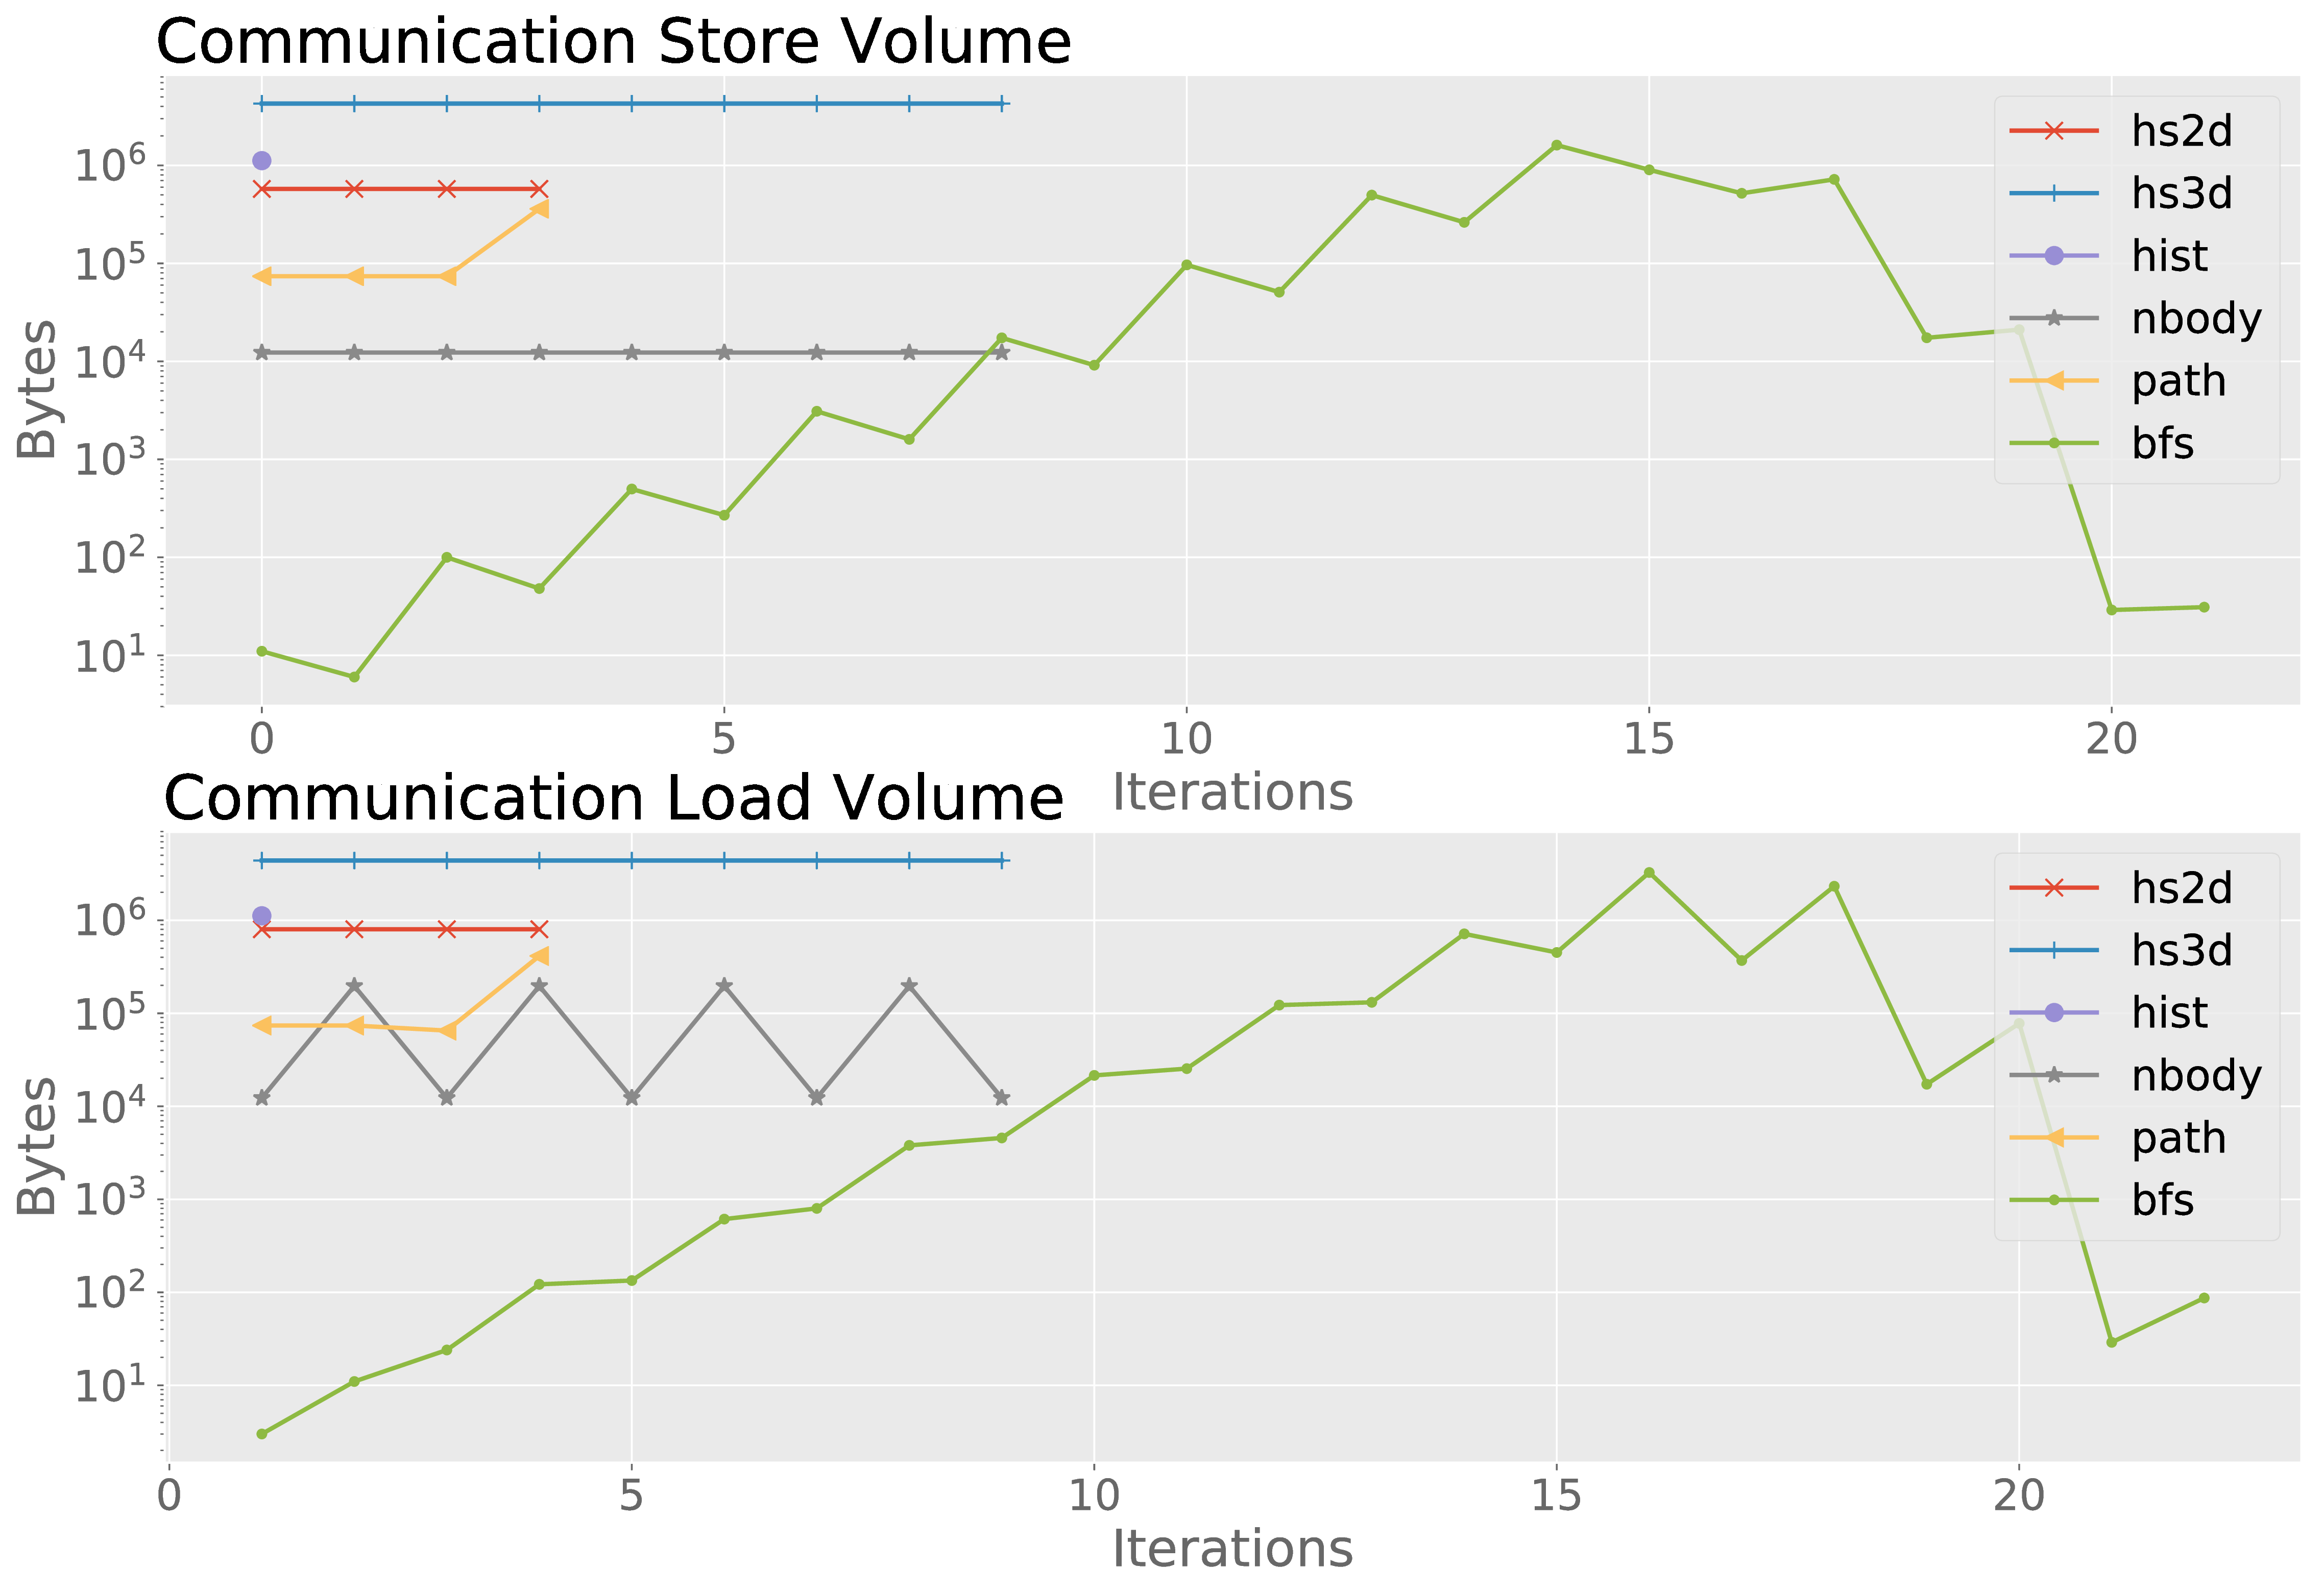
\includegraphics[width=\textwidth]{../../../Global-Memory-Tracing/memtrace-pass/plots/transmission-ratio}
	\caption{Volume of communication loads and stores in each iteration}
	\label{trans-ratio}
\end{figure}
\newpage
\section{Tier III Analysis}
\subsection{Connectivity}
%\subsection{Regularity Evolution}
\begin{figure}[t]
	\centering
		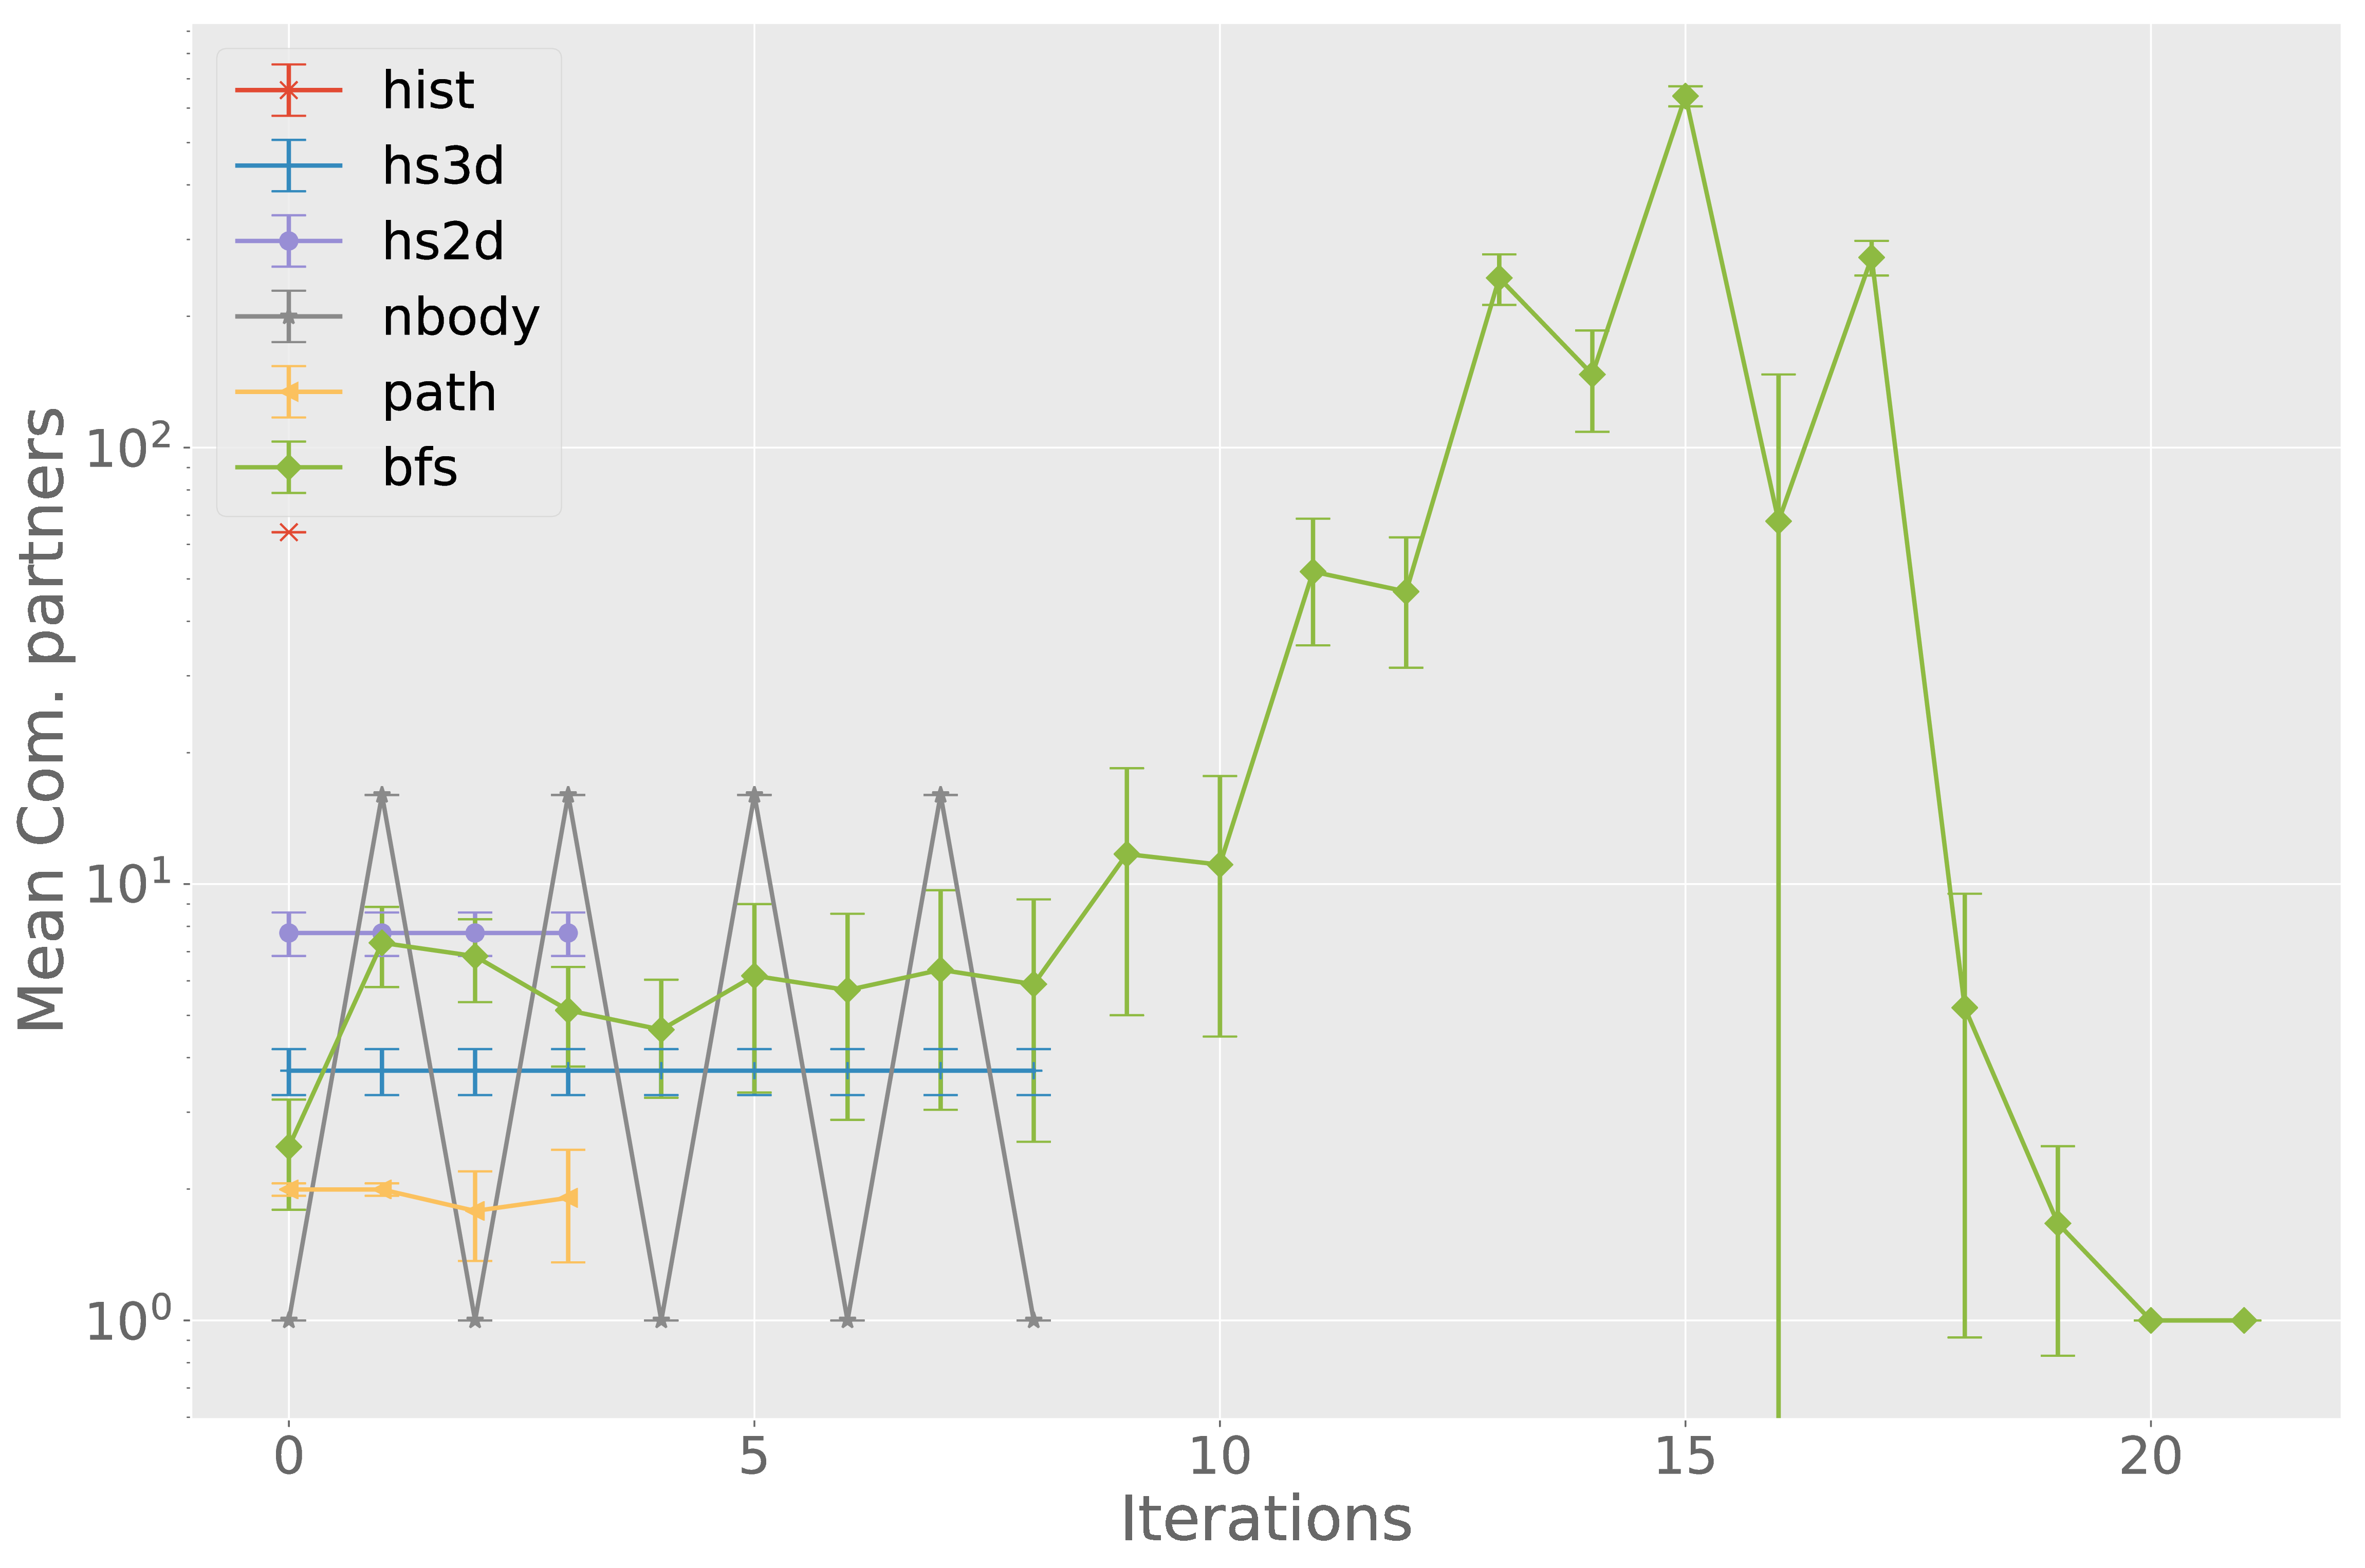
\includegraphics[width=\textwidth]{../../../Global-Memory-Tracing/memtrace-pass/plots/transmission-regularity}
	\caption{Mean connectivity of CTAs, per iteration}
	\label{philandering}
\end{figure}